\chapter{Systemkonzeption}\label{systemkonzeption}

Dieses Kapitel beschreibt die Konzeption des Liveticker-Systems auf Basis der in Kapitel~\ref{motivation-und-anforderungen} hergeleiteten Anforderungen und der in Kapitel~\ref{stand-der-technik} aufgearbeiteten technologischen Grundlagen. Es umfasst Systemüberblick (Abschnitt~\ref{überblick-und-schichtenmodell}), Backend-Konzeption (Abschnitt~\ref{backend-konzeption}), Datenbankkonzeption (Abschnitt~\ref{datenbankkonzeption}), Workflow-Konzeption (Abschnitt~\ref{workflow-konzeption-n8n}), KI-Komponente (Abschnitt~\ref{ki-komponente}), Frontend-Konzeption (Abschnitt~\ref{frontend-konzeption}) sowie Deployment-Konzept (Abschnitt~\ref{deployment-konzept}).



\section{Systemüberblick}\label{überblick-und-schichtenmodell}

Dieser Abschnitt beschreibt das Schichtenmodell (Abschnitt~\ref{schichtenmodell}), die Kommunikations- und Triggerarchitektur (Abschnitt~\ref{kommunikations--und-triggerarchitektur}), das Partner-Team- und White-Label-Konzept (Abschnitt~\ref{partner-team-konzept-und-white-label-steuerung}) sowie den Ticker-Status-Lifecycle und die drei Betriebsmodi (Abschnitt~\ref{status-lifecycle-und-betriebsmodi}).



\subsection{Schichtenmodell}\label{schichtenmodell}

Das System folgt einem Drei-Schichten-Modell, das Integrationslogik, Anwendungslogik und Präsentation klar voneinander trennt. Gegenüber einer Microservices-Architektur reduziert dieses Modell betriebliche Komplexität und Deployment-Overhead, was für ein intern betriebenes Redaktionswerkzeug mit überschaubaren Nutzerzahlen angemessen ist.

Die \textbf{Integrationsschicht} wird durch n8n realisiert und bildet die Schnittstelle zu externen Datenquellen. Sie bindet Football-API, ScorePlay und Social-Feeds an, normalisiert die Rohdaten und kapselt die gesamte Integrationslogik so, dass Workflow-Anpassungen den Anwendungskern nicht berühren. Alle verarbeiteten Daten übergibt n8n ohne eigene Datenpersistenz entweder direkt in die Datenbank oder über REST-Endpunkte an die Anwendungsschicht.

Die \textbf{Anwendungsschicht} basiert auf \texttt{FastAPI} (Python) und PostgreSQL. Sie stellt REST-Schnittstellen bereit, verwaltet Zustandsübergänge der Ticker-Einträge und orchestriert den Großteil der KI-Generierungsschritte, während PostgreSQL alle Domänendaten konsistent speichert. Die Kapselung hinter REST-Schnittstellen abstrahiert die interne Logik von der Präsentationsschicht.

Die \textbf{Präsentationsschicht} ist als mandantenfähiges White-Label-Frontend in React und TypeScript realisiert. Sie deckt den vollständigen Redaktionsworkflow von der Spielauswahl über Prüfung und Bearbeitung bis zur Publikation ab und ist über Instanz, Stil, Sprache und Branding konfigurierbar.

Abbildung~\ref{fig:systemarchitektur} zeigt die drei Schichten mit ihren Technologien und Kommunikationspfaden:

\begin{figure}[H]
\centering
\DiagramSystemArchitektur
\caption{Systemarchitektur: drei Schichten und externe Dienste}
\label{fig:systemarchitektur}
\end{figure}



\subsection{Kommunikations- und
Triggerarchitektur}\label{kommunikations--und-triggerarchitektur}

Die Triggerarchitektur unterscheidet drei Kommunikationsmuster je nach Datenquelle und Betriebskontext. Das System koppelt dabei über drei Schnittstellentypen: \textbf{REST-API} für alle Lese- und Schreiboperationen (Ticker-CRUD, Statusübergänge, manuelle Eingaben), \textbf{n8n-Webhooks} für Stammdaten-Import, Match-Kontext und KI-Generierung sowie den \textbf{WebSocket-Kanal \texttt{/ws/media}} für latenzkritische Medieninhalte.

\textbf{Match-Load.} Der Redakteur navigiert über Land, Team, Wettbewerb und Spieltag zur Spielauswahl, wobei jede Navigationsebene einen n8n-Webhook auslöst, der die zugehörigen Stammdaten von der Football-API abruft und in der Datenbank speichert. Das Frontend liest die Daten anschließend über die REST-API aus der Datenbank aus.

Nach der Spielauswahl gilt für Aufstellungen, Events und Match-Statistiken das Prinzip \textbf{Read first, trigger if missing}: Das Frontend liest zunächst den aktuellen Datenbankstand über die REST-API. Sind die Daten leer, löst es den zugehörigen n8n-Import-Webhook aus. Sobald der Datenzustand befüllt ist, unterbleibt der Webhook-Aufruf bei erneuten Renders. Das Muster greift unabhängig vom Spielstatus, sodass auch abgeschlossene Spiele beim ersten Öffnen vollständig nachgeladen werden. Prematch-Daten und Spieler-Statistiken werden einmalig bei Matchauswahl importiert — unabhängig davon, ob bereits Daten vorliegen, aber ohne Wiederholung bei erneuten Renders.

Beim erstmaligen Öffnen eines Spiels in einer späteren Phase prüft das Frontend zusätzlich, ob Phasen-Drafts für bereits abgeschlossene Spielphasen vorhanden sind. Bei Fehlen löst es einen Catch-up-Endpunkt aus, der die fehlenden Entwürfe nachgeneriert. So findet ein Redakteur, der ein laufendes Spiel erst in der zweiten Halbzeit öffnet, alle Phasen-Drafts vor, ohne manuelle Eingriffe.

\textbf{Live-Betrieb.} Das Frontend triggert Events, Spielstatistiken, Spieler-Statistiken und Minutenupdates bedingungslos im 60-Sekunden-Takt. Die n8n-Workflows führen serverseitig Upserts mit Konfliktbehandlung durch, sodass Mehrfach-Trigger keine Duplikate erzeugen.

\textbf{Interne Workflow-Ketten.} Einzelne n8n-Workflows lösen intern weitere Workflows aus. Der Minuten-Update-Workflow erkennt Spielphasenänderungen und triggert daraufhin den Anpfiff- bzw. Abpfiff-Workflow, der seinerseits die Halbzeit- oder Abpfiff-Zusammenfassung anstößt. Das Frontend ist an dieser Kette nicht beteiligt.

Diese hybride Triggerarchitektur bildet die technische Grundlage für die in Abschnitt~\ref{status-lifecycle-und-betriebsmodi} beschriebenen Betriebsmodi. Für den Ticker-Datenfluss wurde Polling gewählt, da die redaktionelle Latenztoleranz keinen Echtzeit-Push erfordert.

Die folgende Tabelle fasst die Trigger-Muster nach Datenquelle zusammen:

{\def\LTcaptype{none}
\begin{longtable}[]{@{}
  >{\raggedright\arraybackslash}p{(\linewidth - 6\tabcolsep) * \real{0.28}}
  >{\raggedright\arraybackslash}p{(\linewidth - 6\tabcolsep) * \real{0.36}}
  >{\raggedright\arraybackslash}p{(\linewidth - 6\tabcolsep) * \real{0.36}}@{}}
\toprule\noalign{}
Datenquelle & Trigger-Muster & Latenz-Anforderung \\
\midrule\noalign{}
\endhead
\bottomrule\noalign{}
\endlastfoot
Länder, Teams, Wettbewerbe, Spiele & n8n-Webhook (je Navigationsebene, einmalige Initialisierung) & Keine \\
Aufstellungen, Events, Match-Statistiken & „Read first, trigger if missing" (beim Match-Öffnen) & Keine (nur bei leerem Datenbestand) \\
Prematch-Daten, Spieler-Statistiken & Einmalig bei Matchauswahl (unabhängig vom Datenzustand) & $<$30~s (redaktionelle Vorbereitung) \\
Live-Events, Spielstatistiken, Spieler-Statistiken, Minutenupdates & Periodisch, 60-Sekunden-Takt im Live-Betrieb & $<$60~s \\
Medienupdates (ScorePlay) & HTTP POST an \texttt{/media/incoming}; Backend pusht per WebSocket ans Frontend & $<$1~s (Echtzeit) \\
Social-Media-Embeds (Twitter, YouTube, Instagram) & n8n-Webhook (on-demand, redakteurgetriggert) & Keine \\
\end{longtable}
}

\begin{figure}[H]
\centering
\DiagramCommunicationFlow
\caption{Kommunikationsfluss: Frontend, Backend, n8n und externe APIs}
\label{fig:kommunikationsfluss}
\end{figure}



\subsection{Partner-Team-Konzept und
White-Label-Steuerung}\label{partner-team-konzept-und-white-label-steuerung}

Das System unterscheidet zwischen Spielen des Partner-Teams und allen übrigen Spielen. Es erkennt das Partner-Team über ein konfigurierbares Keyword, das in n8n-Workflows und Frontend gegen den Teamnamen abgeglichen wird, unabhängig davon, ob der Verein Heim- oder Auswärtsteam ist. Spiele des Partner-Teams werden der vereinsspezifischen White-Label-Instanz zugeordnet und verwenden standardmäßig den euphorischen Stilmodus (vgl. Abschnitt~\ref{prompt-engineering-strategie}). Dabei werden vereinsspezifische UI-Bereiche eingeblendet, darunter Social-Media-Panels für YouTube, X und Instagram sowie die ScorePlay-Mediensuche für Bildmaterial.

Alle übrigen Spiele durchlaufen die generische Instanz mit neutralem Stil. Für eine neue Instanz sind vier Konfigurationsbereiche anzupassen: \textbf{Frontend-Branding} (Farben, Logo und vereinsspezifische UI-Bereiche), \textbf{Backend-Instanzbezeichner} (interne Kennung für instanzspezifische Filterung und Evaluationsauswertung), \textbf{Few-Shot-Referenzen} (kuratierte Beispieltexte im Zielstil des Vereins) sowie \textbf{n8n-Team-Keyword} (Schlüsselwort zur automatischen Partner-Team-Erkennung in Workflow-Logik und Frontend). Die Implementierungsdetails sind in Kapitel~\ref{implementierung} dokumentiert.



\subsection{Status-Lifecycle und Betriebsmodi}\label{status-lifecycle-und-betriebsmodi}

Jeder Ticker-Eintrag folgt einem Statusmodell mit vier möglichen Zuständen: \texttt{draft} (Entwurf), \texttt{published} (veröffentlicht), \texttt{rejected} (verworfen, terminal) und \texttt{deleted} (weich gelöscht, bleibt in der Datenbank erhalten). Abbildung~\ref{fig:zustandsautomat} zeigt diese Übergänge als Zustandsdiagramm.

\begin{figure}[H]
\centering
\DiagramTickerStates
\caption{Zustandsautomat der Ticker-Einträge (draft, published, rejected, deleted)}
\label{fig:zustandsautomat}
\end{figure}

Eine Rückstufung von \texttt{published} auf \texttt{draft} ist auf drei Wegen möglich. Unmittelbar nach jeder Publikation steht allen Einträgen eine zeitlich begrenzte Widerruf-Aktion zur Verfügung. Phasen- und Zusammenfassungs-Einträge lassen sich darüber hinaus jederzeit über einen einklappbaren Abschnitt im Redaktionspanel zurückziehen. Zusätzlich setzt ein Re-Trigger von Matchphasen-Workflows bestehende Phasen-Einträge automatisch auf \texttt{draft} zurück (vgl. Abschnitt~\ref{n8n-workflow-implementierung}). In allen Fällen kehrt der Eintrag in die redaktionelle Warteschlange zurück und steht zur erneuten Prüfung bereit. Der Übergang \texttt{published} → \texttt{deleted} steht jederzeit zur Verfügung und führt zu einem Soft-Delete. Der Zustand \texttt{rejected} ist terminal und führt nicht zu einem physischen Datenbankdeletion. Abgelehnte Einträge verbleiben mit ihrem Status in der Datenbank, um die Reproduzierbarkeit späterer Qualitätsauswertungen zu gewährleisten. Das Feld \texttt{source} (\texttt{ai} vs.~\texttt{manual}) und das Feld \texttt{instance} (\texttt{ef\_whitelabel} / \texttt{generic}) ergänzen jeden Eintrag um Herkunfts- und Instanzattributierung, die für instanzspezifische Few-Shot-Filterung und reproduzierbare Evaluationsauswertungen genutzt wird.

Das Feld \texttt{ticker\_mode} in \texttt{matches} steuert das Verhalten der Generierungspipeline pro Spiel und ist zur Laufzeit umschaltbar. Im Modus \textbf{\texttt{auto}} (vollautomatisch) läuft die Triggerkette ohne redaktionellen Eingriff. KI-Ergebnisse werden direkt veröffentlicht. Für Robustheit sind zwei parallele Publikationspfade konzipiert: Der primäre Pfad verläuft über n8n, der sekundäre Pfad ist ein Frontend-seitiger Fallback, der neu eintreffende Entwürfe unmittelbar publiziert — etwa bei verzögerten n8n-Webhooks oder bei Modusumschaltung im Frontend ohne n8n-Neustart. Im Modus \textbf{\texttt{coop}} (kooperativ, Human-in-the-Loop) erzeugt die KI Entwürfe, über deren Freigabe oder Ablehnung die Redaktion entscheidet. Dieser Modus bildet das primäre Zielbild des Systems. Im Modus \textbf{\texttt{manual}} (rein redaktionell) werden Einträge ausschließlich manuell erstellt. Eingehende Events lösen nur die Datenpersistenz aus, nicht die LLM-Pipeline. Abbildung~\ref{fig:betriebsmodi} stellt alle drei Modi vergleichend gegenüber.

\begin{figure}[H]
\centering
\DiagramBetriebsmodi
\caption[Die drei Betriebsmodi im Überblick]{Die drei Betriebsmodi im Überblick: Automatisierungsgrad und Entscheidungshoheit je Modus}
\label{fig:betriebsmodi}
\end{figure}



\section{Backend-Konzeption}\label{backend-konzeption}

Das \texttt{FastAPI}-Backend realisiert die Anwendungslogik des Systems. Die folgenden Abschnitte behandeln Framework-Wahl (Abschnitt~\ref{framework-wahl}), interne Schichtstruktur (Abschnitt~\ref{interne-schichtstruktur}), API-Design (Abschnitt~\ref{api-design-und-endpunktstrategie}) sowie das Qualitätssicherungskonzept (Abschnitt~\ref{qualitätssicherungskonzept}).

\subsection{Framework-Wahl}\label{framework-wahl}

Als Backend-Framework wurde \texttt{FastAPI} gewählt (vgl. Abschnitt~\ref{backend-framework-und-persistenzschicht}). Die native asyncio-Unterstützung ermöglicht parallele LLM- und API-Aufrufe ohne Blockierung, die Pydantic-Integration sichert typisierte Schnittstellen zwischen Frontend, Backend und n8n. Ein konfigurierbarer Semaphore-Mechanismus begrenzt dabei die Anzahl gleichzeitiger LLM-Aufrufe und verhindert Rate-Limit-Überschreitungen bei parallelen Spielen.

\subsection{Interne Schichtstruktur}\label{interne-schichtstruktur}

Die interne Schichtstruktur folgt dem \textbf{Repository Pattern} (Fowler 2002, S.~322) und gliedert sich in fünf Komponenten: \textbf{Router} (HTTP-Schicht, Anfrage-Orchestrierung), \textbf{Service} (Domänenlogik und Orchestrierung komplexer Abläufe), \textbf{Repository} (gekapselter Datenbankzugriff), \textbf{ORM-Modell} (Persistenzstruktur) und \textbf{Pydantic-Schema} (typisierte API-Verträge zwischen den Schichten).

Die Ablaufmuster unterscheiden sich je nach Komplexität der Operation. Einfache CRUD-Operationen folgen dem direkten Muster Router \(\rightarrow\) Repository. Komplexere Generierungs- und Orchestrierungsabläufe durchlaufen zusätzlich die Service-Schicht: Router \(\rightarrow\) Service \(\rightarrow\) Repository. Diese Trennung ermöglicht transaktionale Testbarkeit, da Repositories in Tests mit echten Datenbanktransaktionen geprüft und nach jedem Test zurückgerollt werden können. Als explizite Layering-Einschränkung gilt dabei, dass der LLM-Service keine Datenbankabhängigkeit trägt — Datenbankzugriff erfolgt ausschließlich über die Repository-Schicht.



\subsection{API-Design und
Endpunktstrategie}\label{api-design-und-endpunktstrategie}

Die Backend-Schnittstelle ist als versionierte REST-API unter \texttt{/api/v1} ausgelegt (vgl. Fielding 2000, Kap.~5). Ressourcen wie \texttt{teams}, \texttt{matches}, \texttt{ticker} und \texttt{media} bilden eigenständige Endpunkte und folgen einheitlichen HTTP-Methodenkonventionen. Das Design trennt Datenendpunkte von Triggerendpunkten: Leseoperationen bleiben seiteneffektfrei, während Import- und Generierungsprozesse über dedizierte Triggerendpunkte ausgelöst werden. Die Pydantic-Schemas dienen dabei gleichzeitig als API-Verträge und als Grundlage für die automatisch generierte OpenAPI-Dokumentation, sodass Frontend und n8n die Schnittstelle ohne manuelle Dokumentation nachvollziehen können. Die konkrete Endpunktstruktur ist in Abschnitt~\ref{api-router-endpunktstruktur} dokumentiert.




\subsection{Qualitätssicherungskonzept}\label{qualitätssicherungskonzept}

Die Qualitätssicherung folgt dem Testpyramiden-Modell nach Cohn (2009). Schnelle, granulare Unit-Tests bilden die Basis. Integrationstests prüfen das Zusammenspiel über Komponentengrenzen. Eine schlanke E2E-Schicht validiert kritische Nutzerpfade im Browser. Das Verhältnis der Testebenen ist dabei kostenbewusst gestaltet. Teure E2E-Tests decken nur Regressionsrisiken mit hoher Nutzerauswirkung ab, während die eigentliche Logik über Unit- und API-Tests gesichert ist. Externe Dienste wie LLM-Provider werden durch deterministisch kontrollierbare Mock-Implementierungen ersetzt, da echte Aufrufe in automatisierten Läufen nicht reproduzierbar sind. Das Pyramidenmodell gilt systemweit, die frontend-spezifischen Testebenen und Werkzeuge sind in Abschnitt~\ref{frontend-teststrategie} beschrieben.




\section{Datenbankkonzeption}\label{datenbankkonzeption}

Die Persistenzschicht des Systems basiert auf PostgreSQL. Die folgenden Abschnitte begründen die Datenbankwahl (Abschnitt~\ref{datenbankwahl}), beschreiben die Schemadesign-Prinzipien (Abschnitt~\ref{schemadesign-prinzipien}) und erläutern die Migrationsstrategie (Abschnitt~\ref{migrationsstrategie}).

\subsection{Datenbankwahl}\label{datenbankwahl}

Als Datenbanksystem wurde PostgreSQL gewählt. Die Domänendaten weisen eine stark relationale Struktur auf: Teams, Wettbewerbe, Spiele, Events und Ticker-Einträge sind durch Fremdschlüsselbeziehungen verbunden und erfordern referenzielle Integrität sowie ACID-konforme Zustandsübergänge, was relationale Systeme gegenüber dokumentenorientierten Alternativen vorzieht (vgl. Abschnitt~\ref{backend-framework-und-persistenzschicht}). PostgreSQL bietet darüber hinaus native JSONB-Unterstützung und upsertfähige Konfliktbehandlung, die für die Schemadesign-Entscheidungen in Abschnitt~\ref{schemadesign-prinzipien} genutzt werden. Als ORM kommt synchrones SQLAlchemy zum Einsatz, da Datenbankoperationen im vorliegenden System kurzläufig sind und ein asynchrones ORM Komplexität ohne erwartbaren Latenz-Vorteil hinzufügen würde.

\subsection{Schemadesign-Prinzipien}\label{schemadesign-prinzipien}

Das Schema folgt einem hybriden Entwurfsansatz aus strukturierter Normalisierung und gezielter Schemaflexibilität. Abbildung~\ref{fig:er-diagramm} zeigt die zentralen Entitäten und ihre Beziehungen. Das Diagramm zeigt die FK-verbundenen Kerntabellen; \texttt{media\_queue}, \texttt{style\_references} und \texttt{settings} sind aus Übersichtlichkeitsgründen nicht dargestellt.

\begin{figure}[H]
  \centering
  \DiagramDataModel
  \caption{Vereinfachtes ER-Diagramm der zentralen Systemtabellen (konzeptionell)}
  \label{fig:er-diagramm}
\end{figure}

Die zentralen Domänenobjekte (\texttt{teams}, \texttt{matches}, \texttt{events}, \texttt{ticker\_entries}, \texttt{players}, \texttt{competitions}) sind normalisiert modelliert, um Redundanzen zu minimieren sowie Integrität und Auswertbarkeit im Live-Betrieb stabil zu halten. Statistiktabellen sind über explizite Spalten modelliert, um konsistente Abfragen und robuste Aggregationen zu ermöglichen.

Stammdaten-Entitäten führen drei Schlüsselfelder: einen numerischen Primärschlüssel für performante Datenbankjoins, einen numerischen Fremdbezeichner der Football-API für idempotentes Upsert-Matching bei Reimports sowie eine UUID als stabilen Referenzschlüssel für externe API-Konsumenten. Diese Trennung entkoppelt interne Datenbankidentität, Datenquellen-Matching und externe Exposition voneinander.

Abhängige Entitäten wie Events und Ticker-Einträge sind per Fremdschlüssel-Kaskade an das übergeordnete Spiel gebunden. Das Löschen eines Spiels entfernt konsistent alle zugehörigen Daten, ohne manuelle Bereinigungsschritte zu erfordern.

JSONB-Felder kommen in zwei Fällen zum Einsatz: für mehrsprachige Anzeigefelder mit variablen Sprachschlüsseln (z.\,B. \texttt{localized\_title}) sowie für dynamische Kontextstrukturen, deren Schema je nach Ereignistyp variiert (z.\,B. Vorabend- und Kopf-an-Kopf-Daten in \texttt{synthetic\_events}). Damit bleibt die JSONB-Nutzung auf begründete Ausnahmen beschränkt, während der Großteil des Schemas typisiert und abfrageoptimiert bleibt.

Stammdaten-Entitäten werden bei wiederholtem Import aktualisiert (Upsert), Ereignisentitäten hingegen unverändert belassen, da sie den historischen Spielverlauf abbilden. Die konkreten Implementierungsdetails sind in Abschnitt~\ref{datenmodelle-datenbankschema-und-api-validierung} dokumentiert.

\subsection{Migrationsstrategie}\label{migrationsstrategie}

Schemaänderungen werden über \textbf{Alembic} versioniert, das als dediziertes Migrationswerkzeug für SQLAlchemy (vgl. Abschnitt~\ref{datenbankwahl}) konzipiert ist. Die enge SQLAlchemy-Integration ermöglicht die automatische Ableitung von Migrationsdateien aus ORM-Modelländerungen und vermeidet damit eine Bruchstelle zwischen Datenbankschema und Anwendungsmodell, die bei werkzeugfremden Alternativen entsteht. Jede Schemaänderung wird als versionierte Migrationsdatei abgelegt, die sequenziell anwendbar und rückrollbar ist. Neue Instanzen werden durch sequenzielle Migration auf den aktuellen Schemastand gebracht, ohne manuelle Eingriffe in die Datenbankstruktur zu erfordern.

Das persistierte Datenmodell bildet die Grundlage für die darüberliegende Workflow-Schicht, die alle Datenimporte und Generierungsprozesse orchestriert.

\section{Workflow-Konzeption (n8n)}\label{workflow-konzeption-n8n}

n8n übernimmt als Orchestrierungsschicht alle Datenimport- und Generierungsprozesse. Abschnitt~\ref{n8n-technologiewahl} begründet die Technologiewahl, Abschnitt~\ref{n8n-designprinzipien} legt die übergreifenden Designprinzipien fest und Abschnitt~\ref{workflow-klassen} beschreibt die resultierenden Workflow-Klassen.

\subsection{Technologiewahl}\label{n8n-technologiewahl}

Gegenüber Batch-orientierten Alternativen wie Apache Airflow und Prefect, die prozedurale Python-Kenntnisse für jeden Workflow voraussetzen, ermöglicht n8n die grafische Komposition aus typisierten Knoten (vgl. Abschnitt~\ref{etl-prozesse-und-workflow-automatisierung}; Venkiteela 2025, S.~2--3). Native Postgres-Knoten und Code-Knoten für benutzerdefiniertes JavaScript decken den systemspezifischen Bedarf an direktem Datenbankzugriff und Transformationslogik ab, während die Unterstützung sowohl Webhook-getriggerter als auch zeitgesteuerter Workflows in einer Umgebung die in Abschnitt~\ref{kommunikations--und-triggerarchitektur} beschriebene hybride Triggerarchitektur ohne zusätzliche Infrastruktur abbildet.

\subsection{Designprinzipien}\label{n8n-designprinzipien}

Alle Workflows sind auf wiederholten, bedingungslosen Aufruf ausgelegt. Datenbankoperationen nutzen \texttt{ON CONFLICT}-Strategien; Generierungs-Workflows prüfen vor jedem LLM-Aufruf, ob bereits ein Ticker-Eintrag für das auslösende Ereignis existiert. Dieses Idempotenz-Prinzip verhindert redundante LLM-Aufrufe und Dateninkonsistenzen unabhängig davon, wie oft ein Workflow ausgelöst wird.

Für den Datenbankzugriff gilt eine klare Trennung: Reine Datenimporte schreibt n8n direkt per SQL in die Datenbank, um HTTP-Overhead zu vermeiden. Ereignis-basierte Generierung und Phasenübergänge werden als REST-Aufrufe ans Backend delegiert, das die zugehörige Geschäftslogik kapselt. Zusammenfassungs-Workflows bauen ihren Prompt aus mehreren Datenquellen selbst zusammen und rufen den LLM-Provider direkt auf, da sie größere Kontextmengen aus Spielstand, Events, Statistiken und Aufstellungen verarbeiten als der standardisierte Generierungsendpunkt voraussetzt.

Die Betriebsmodus-Entscheidung liegt bei n8n. Vor jedem Generierungsaufruf liest der Workflow \texttt{ticker\_mode} aus der Datenbank und übergibt \texttt{auto\_publish} als Binärparameter an den Generierungsendpunkt. Das Backend bleibt dadurch modusunabhängig; die Entscheidung über den Automatisierungsgrad trifft allein n8n auf Basis des konfigurierten Spielmodus (vgl. Abschnitt~\ref{status-lifecycle-und-betriebsmodi}).

\subsection{Workflow-Klassen}\label{workflow-klassen}

Die 17 Workflows folgen zwei strukturell unterschiedlichen Mustern. Event-basierte Generierungs-Workflows prüfen vor jedem LLM-Aufruf, ob das auslösende Ereignis bereits persistiert ist, und sind damit idempotent gegenüber dem bedingungslosen Polling-Takt des Frontends (vgl. Abschnitt~\ref{kommunikations--und-triggerarchitektur}). Zusammenfassungs- und Monitoring-Workflows folgen einem direkten Pfad ohne Abgleich, da sie einmalig pro Spielphase ausgelöst werden. Die folgende Übersicht zeigt alle 17 Workflows gegliedert nach sechs funktionalen Klassen:

{\def\LTcaptype{none} % do not increment counter
\begin{longtable}[]{@{}
  >{\raggedright\arraybackslash}p{(\linewidth - 4\tabcolsep) * \real{0.2727}}
  >{\raggedright\arraybackslash}p{(\linewidth - 4\tabcolsep) * \real{0.4091}}
  >{\raggedright\arraybackslash}p{(\linewidth - 4\tabcolsep) * \real{0.3182}}@{}}
\toprule\noalign{}
\begin{minipage}[b]{\linewidth}\raggedright
Gruppe
\end{minipage} & \begin{minipage}[b]{\linewidth}\raggedright
Workflows
\end{minipage} & \begin{minipage}[b]{\linewidth}\raggedright
Trigger
\end{minipage} \\
\midrule\noalign{}
\endhead
\bottomrule\noalign{}
\endlastfoot
\textbf{A) Stammdaten} & Countries, Teams, Competitions, Matches & Bei leeren Daten \\
\textbf{B) Matchdaten} & Lineups, Match-/Spielerstatistiken, Prematch & Nach Matchauswahl; Statistiken periodisch im Live-Betrieb \\
\textbf{C) KI-Generierung} & Events-LLM, Halbzeit-/Abpfiff-Zusammenfassung, Anpfiff/Abpfiff & Modus- und Event-gesteuert \\
\textbf{D) Medien \& Social} & ScorePlay, Twitter/X, YouTube, Instagram & Mediensuche \\
\textbf{E) Monitoring} & Live-Stats-Monitor & Spieltag-gesteuert \\
\textbf{F) Spielzeit} & Minutenupdate & Webhook \\
\end{longtable}
}

Die Aufteilung in Workflow-Klassen reduziert Kopplung und erlaubt es, einzelne Teilprozesse unabhängig anzupassen. Die konkreten Implementierungen sind in Abschnitt~\ref{n8n-workflow-implementierung} dokumentiert.






\section{KI-Komponente}\label{ki-komponente}

Die LLM-gestützte Textgenerierung ist als providerunabhängige Komponente mit konfigurierbarer Prompt-Strategie konzipiert. Sie umfasst die Multi-Provider-Architektur (Abschnitt~\ref{multi-provider-architektur}), die Prompt-Engineering-Strategie (Abschnitt~\ref{prompt-engineering-strategie}) und das Mehrsprachigkeitskonzept (Abschnitt~\ref{mehrsprachige-textgenerierung-konzept}).

\subsection{Multi-Provider-Architektur}\label{multi-provider-architektur}

Die KI-Komponente ist als providerunabhängige Abstraktionsschicht konzipiert, in der der LLM-Dienst OpenRouter, Google Gemini, OpenAI, Anthropic und einen Mock-Provider hinter einer einheitlichen internen Schnittstelle kapselt. Das System setzt primär \textbf{OpenRouter} als Gateway ein, weil es Modelle zahlreicher Anbieter über einen einzigen API-Zugang zugänglich macht und der Modellwechsel damit lediglich eine Konfigurationsänderung erfordert, was Modellvergleiche auf demselben Prompt erleichtert (vgl. Abschnitte~\ref{large-language-models} und~\ref{llm-service-prompt-aufbau-und-provider-dispatch}). Eine Fallback-Kette aktiviert beim Start den ersten Anbieter mit konfiguriertem API-Key (openrouter $\rightarrow$ gemini $\rightarrow$ openai $\rightarrow$ anthropic $\rightarrow$ mock). Als direkter Anthropic-Fallback ohne OpenRouter-Intermediär dient Claude Haiku, das für Kurztext-Aufgaben niedrige Latenzen bei geringen Kosten erzielt und Konfigurationsszenarien ohne OpenRouter-Zugang absichert. Ist kein API-Key konfiguriert, übernimmt der Mock-Provider und sichert die Lauffähigkeit für Entwicklung und Tests.

Als Standardmodell im Deployment wurde \textbf{Gemini 2.0 Flash Lite} über OpenRouter gewählt. Die Entscheidung folgt aus Aufgabencharakteristik und Kosteneffizienz. Liveticker-Texte sind kurz und faktenbasiert, weshalb kompakte Modelle vergleichbare Qualität bei deutlich niedrigerer Latenz erzielen. Zudem zählt das Modell zu den kostengünstigsten kommerziell verfügbaren Optionen und macht den Dauerbetrieb über eine Saison für ressourcenbegrenzte Redaktionen wirtschaftlich darstellbar (vgl. Abschnitt~\ref{redaktioneller-aufwand-bei-livetickern}).




\subsection{Prompt-Engineering-Strategie}\label{prompt-engineering-strategie}

Die in Abschnitt~\ref{linguistische-anforderungen-an-die-textgenerierung} hergeleiteten Merkmale des Liveticker-Genres (konzeptionelle Mündlichkeit, Ellipsen-Syntax, Präsenstempus, Graphostilistik und direkte Adressierung) definieren das Zielformat, auf das das LLM konditioniert wird. Der Regelblock des Prompts operationalisiert diese Vorgaben als explizite Modellanweisungen.

Die Generierung verwendet ein modulares Prompt-Design mit sechs Bausteinen (Rolleninstruktion, Stilinstruktion, Faktenblock, Kontextblock, Few-Shot-Block und Regelblock), die dynamisch zusammengesetzt werden und deren Zusammenspiel Abbildung~\ref{fig:prompt-aufbau} zeigt. Die Stilinstruktion parametrisiert eines von drei Stilprofilen — \textbf{neutral} (sachlicher, unparteiischer Reporter-Stil), \textbf{euphorisch} (leidenschaftlicher Fan-Stil, vereinsspezifisch personalisiert durch explizite Nennung des Partnervereins in der Stilinstruktion) und \textbf{kritisch} (analytischer Kommentator-Stil mit expliziter Fehlerbenennung). Der Few-Shot-Block ist instanzspezifisch und wird nur eingebettet, wenn für die aktive Instanz Stilreferenzen in der Datenbank hinterlegt sind.

\begin{figure}[H]
\centering
\DiagramPromptPipeline
\caption{Prompt-Aufbau: Eingaben, Prompt-Bausteine, LLM-Aufruf und Ticker-Text}
\label{fig:prompt-aufbau}
\end{figure}

Der Few-Shot-Block wird aus manuell kuratierten Original-Tickertexten des Partnervereins gespeist. Pro LLM-Aufruf werden bis zu drei Referenzen zufällig aus dem nach Ereignistyp, Instanz und optional Liga gefilterten Pool selektiert. Die Randomisierung verhindert die monotone Reproduktion identischer Formulierungen bei gleichartigen Events, während der stilistische Korridor gewahrt bleibt. Für Pre-Match-Typen enthält der Prompt zusätzliche Restriktionen, um Halluzinationen von Live-Szenen zu vermeiden und die Ausgabe auf Vorschau- und Analyseinhalte zu begrenzen. Die konkreten Inferenzparameter sind in Abschnitt~\ref{llm-service-prompt-aufbau-und-provider-dispatch} dokumentiert.

Die Generierungspipeline folgt einer asymmetrischen Idempotenz-Strategie. Für ereignisbasierte Generierung prüft der Pipeline-Einstiegspunkt, ob bereits ein aktiver Ticker-Eintrag für das auslösende Ereignis existiert, und überspringt den LLM-Aufruf in diesem Fall. Für synthetische Spielphasen-Events unterbleibt diese Prüfung bewusst: Da Phasen-Workflows denselben Auslöser wiederholen, würde ein Dedup-Schutz eine Neugenerierung nach redaktioneller Ablehnung dauerhaft blockieren. Abgelehnte Phasen-Drafts erscheinen damit beim nächsten Workflow-Lauf automatisch neu.

\subsection{Mehrsprachige Textgenerierung}\label{mehrsprachige-textgenerierung-konzept}

Mehrsprachigkeit ist als eines der drei zentralen Systemziele in der Forschungsfrage verankert (vgl. Abschnitt~\ref{forschungsfrage}) und adressiert den internationalen Spielbetrieb des Partnervereins in europäischen Wettbewerben (vgl. Abschnitt~\ref{mehrsprachigkeit-als-herausforderung}). Mehrsprachigkeit wird als natives Merkmal der Generierungspipeline konzipiert, nicht als nachträgliche Übersetzungsschicht. Das vermeidet eine separate Übersetzungsinfrastruktur und stellt sicher, dass stilistische Anforderungen direkt in der Zielsprache umgesetzt werden.

Das System unterstützt Deutsch, Englisch, Spanisch und Französisch, die Zielsprache wählt der Redakteur zur Laufzeit. Für bereits bestehende Einträge des aktiven Spiels greift ein Batch-Übersetzungsendpunkt. Derselbe Prompt-Mechanismus gilt für alle Sprachen ohne sprachspezifische Varianten. Generierung und Übersetzung folgen dabei unterschiedlichen Temperaturregimen: Die Generierung verwendet eine höhere Temperatur für stilistische Variation, die Übersetzung eine niedrige deterministische Temperatur, um reproduzierbare und sprachlich konsistente Ergebnisse zu erzielen. Die konkrete Implementierung ist in den Abschnitten~\ref{api-router-endpunktstruktur} und~\ref{llm-service-prompt-aufbau-und-provider-dispatch} dokumentiert.

\section{Frontend-Konzeption}\label{frontend-konzeption}

Das React-Frontend ist auf mandantenfähigen White-Label-Betrieb ausgelegt. Die Konzeption gliedert sich in Framework-Wahl (Abschnitt~\ref{frontend-framework-wahl}), Architektur und Zustandsmanagement (Abschnitt~\ref{architekturprinzipien}), Layout und Moduslogik (Abschnitt~\ref{dreispalten-layout-und-redaktionsfluss}), UI-Design und visuelles Branding (Abschnitt~\ref{ui-design-branding}) sowie Teststrategie (Abschnitt~\ref{frontend-teststrategie}).

\subsection{Framework-Wahl}\label{frontend-framework-wahl}

React wurde gegenüber Vue und Svelte bevorzugt (vgl. Abschnitt~\ref{frontend-framework}). Das Hook-Modell kapselt Zustand, Seiteneffekte und Echtzeitkommunikation pro Komponente und ermöglicht so die wiederverwendbaren Custom Hooks, auf denen die Architektur aus Abschnitt~\ref{architekturprinzipien} aufbaut.

\subsection{Architektur und Zustandsmanagement}\label{architekturprinzipien}

Das Frontend trennt UI-Komponenten, datenbezogene Hooks und API-Zugriffsschicht klar voneinander. Auf eine globale State-Management-Bibliothek wie Redux oder Zustand wurde bewusst verzichtet, da der Zustandsumfang des Redaktionsworkflows keine zusätzliche Abstraktion rechtfertigt. Gemeinsamer Zustand für tief verschachtelte Komponenten wird über dedizierte Context-Provider bereitgestellt, um Prop-Drilling zu vermeiden und Re-Renders zu kontrollieren. Die Zustands- und Interaktionslogik ist in wiederverwendbare Custom Hooks aufgeteilt, die Navigation, Polling, Echtzeitkommunikation und Redaktionsinteraktion abdecken. Die Hooks sind in zwei Ebenen organisiert: allgemein wiederverwendbare Hooks unter \texttt{src/hooks/} und feature-spezifische Hooks unter \texttt{components/LiveTicker/hooks/}, um Kopplung zwischen Kernarchitektur und Ticker-Feature-Logik zu begrenzen. Zustandsänderungen mit sichtbarer Latenz — insbesondere die Modusumschaltung per PATCH-Aufruf — werden über Optimistic-Updates realisiert: Der UI-Zustand wird sofort lokal gesetzt, während die Backend-Synchronisation im Hintergrund läuft. Die White-Label-Fähigkeit ist über eine Konfigurationsschicht konzipiert, die Farben, Team-Keyword und API-Endpunkte je Instanz variiert (vgl. Abschnitt~\ref{komponentenhierarchie}).

Der Context ist bewusst in einen Daten-Context und einen Aktions-Context aufgeteilt. Komponenten, die nur Aktionen konsumieren, re-rendern damit nicht bei jeder Datenaktualisierung — ein relevanter Performance-Gewinn beim 15-Sekunden-Polling-Takt des Live-Betriebs.

Jedes der drei Panels ist von einer eigenen \texttt{ErrorBoundary}-Instanz umschlossen. Ein unkontrollierter Rendering-Fehler in einem Panel blockiert damit nicht die übrigen Panels und hält die Redaktionsoberfläche auch bei partiellen Fehlern arbeitsfähig.

\subsection{Layout und Moduslogik}\label{dreispalten-layout-und-redaktionsfluss}

Die Hauptansicht folgt einem Dreispalten-Ansatz mit klarer Aufgabenverteilung. Das linke Panel zeigt den chronologischen Feed publizierter Ticker-Einträge. Das mittlere Panel bildet die redaktionelle Kernarbeit ab, darunter Event-Verarbeitung in Abhängigkeit vom Betriebsmodus, Draft-Prüfung und Freigabe, manuelle Eingabe sowie integrierte Media- und Social-Panels für Partnervereinsspiele. Das rechte Panel liefert Kontextinformationen wie Matchstatistiken, Aufstellungen und spielerbezogene Leistungsdaten.

Die Modusumschaltung ist mit Bestätigungsdialog und visueller Rückmeldung ausgestattet. Für einen tastaturgesteuerten Redaktionsfluss ohne Mauswechsel sind drei Shortcut-Ebenen konzipiert: \texttt{Ctrl+1} / \texttt{Ctrl+2} / \texttt{Ctrl+3} schalten global zwischen den drei Betriebsmodi um; \texttt{TAB} und \texttt{ESC} lösen im kooperativen Modus Accept bzw. Reject eines Entwurfs aus (vgl. Abschnitt~\ref{status-lifecycle-und-betriebsmodi}); \texttt{?} öffnet ein Keyboard-Hints-Modal mit einer kontextsensitiven Übersicht aller aktiven Shortcuts und Slash-Commands. Im Auto-Modus wird das mittlere Panel ausgeblendet; das Layout wechselt von drei auf zwei Spalten, da ohne redaktionellen Eingriff kein Editierbereich benötigt wird. Die Spaltenbreiten sind per Drag-to-Resize stufenlos anpassbar, um den Arbeitsbereich auf unterschiedliche Bildschirme und Präferenzen abzustimmen.

Für die manuelle Eingabe ist ein \textbf{Slash-Command-Parser} konzipiert. Phase- und Event-Commands (\texttt{/anpfiff}, \texttt{/goal}, \texttt{/gelb} u.\,a.) werden über eine einheitliche Syntaxstruktur geparst und direkt in strukturierte Ticker-Einträge überführt, ohne Formularnavigation.

Das Layout ist vollständig responsiv ausgelegt. Auf mobilen Geräten kollabiert die Dreispalten-Ansicht auf eine Einspalten-Darstellung mit einer Bottom-Tab-Leiste, über die zwischen Ticker-Feed, Editor und Statistik-Panel gewechselt wird. Die konkreten Implementierungen sind in Abschnitt~\ref{frontend-implementierung} dokumentiert.

\subsection{UI-Design und visuelles Branding}\label{ui-design-branding}

Vor der Implementierung wurde die Benutzeroberfläche vollständig in \textbf{Figma} als interaktiver Prototyp entworfen. Die Wireframes definierten das Drei-Spalten-Layout, den Redaktionsfluss und die Zustandsdarstellungen der Ticker-Einträge, sodass Layoutentscheidungen bereits vor der ersten React-Komponente validiert waren. Abbildung~\ref{fig:figma-wireframe} zeigt den Prototyp-Stand, der als Vorlage für die Implementierung diente.

\begin{figure}[H]
\centering
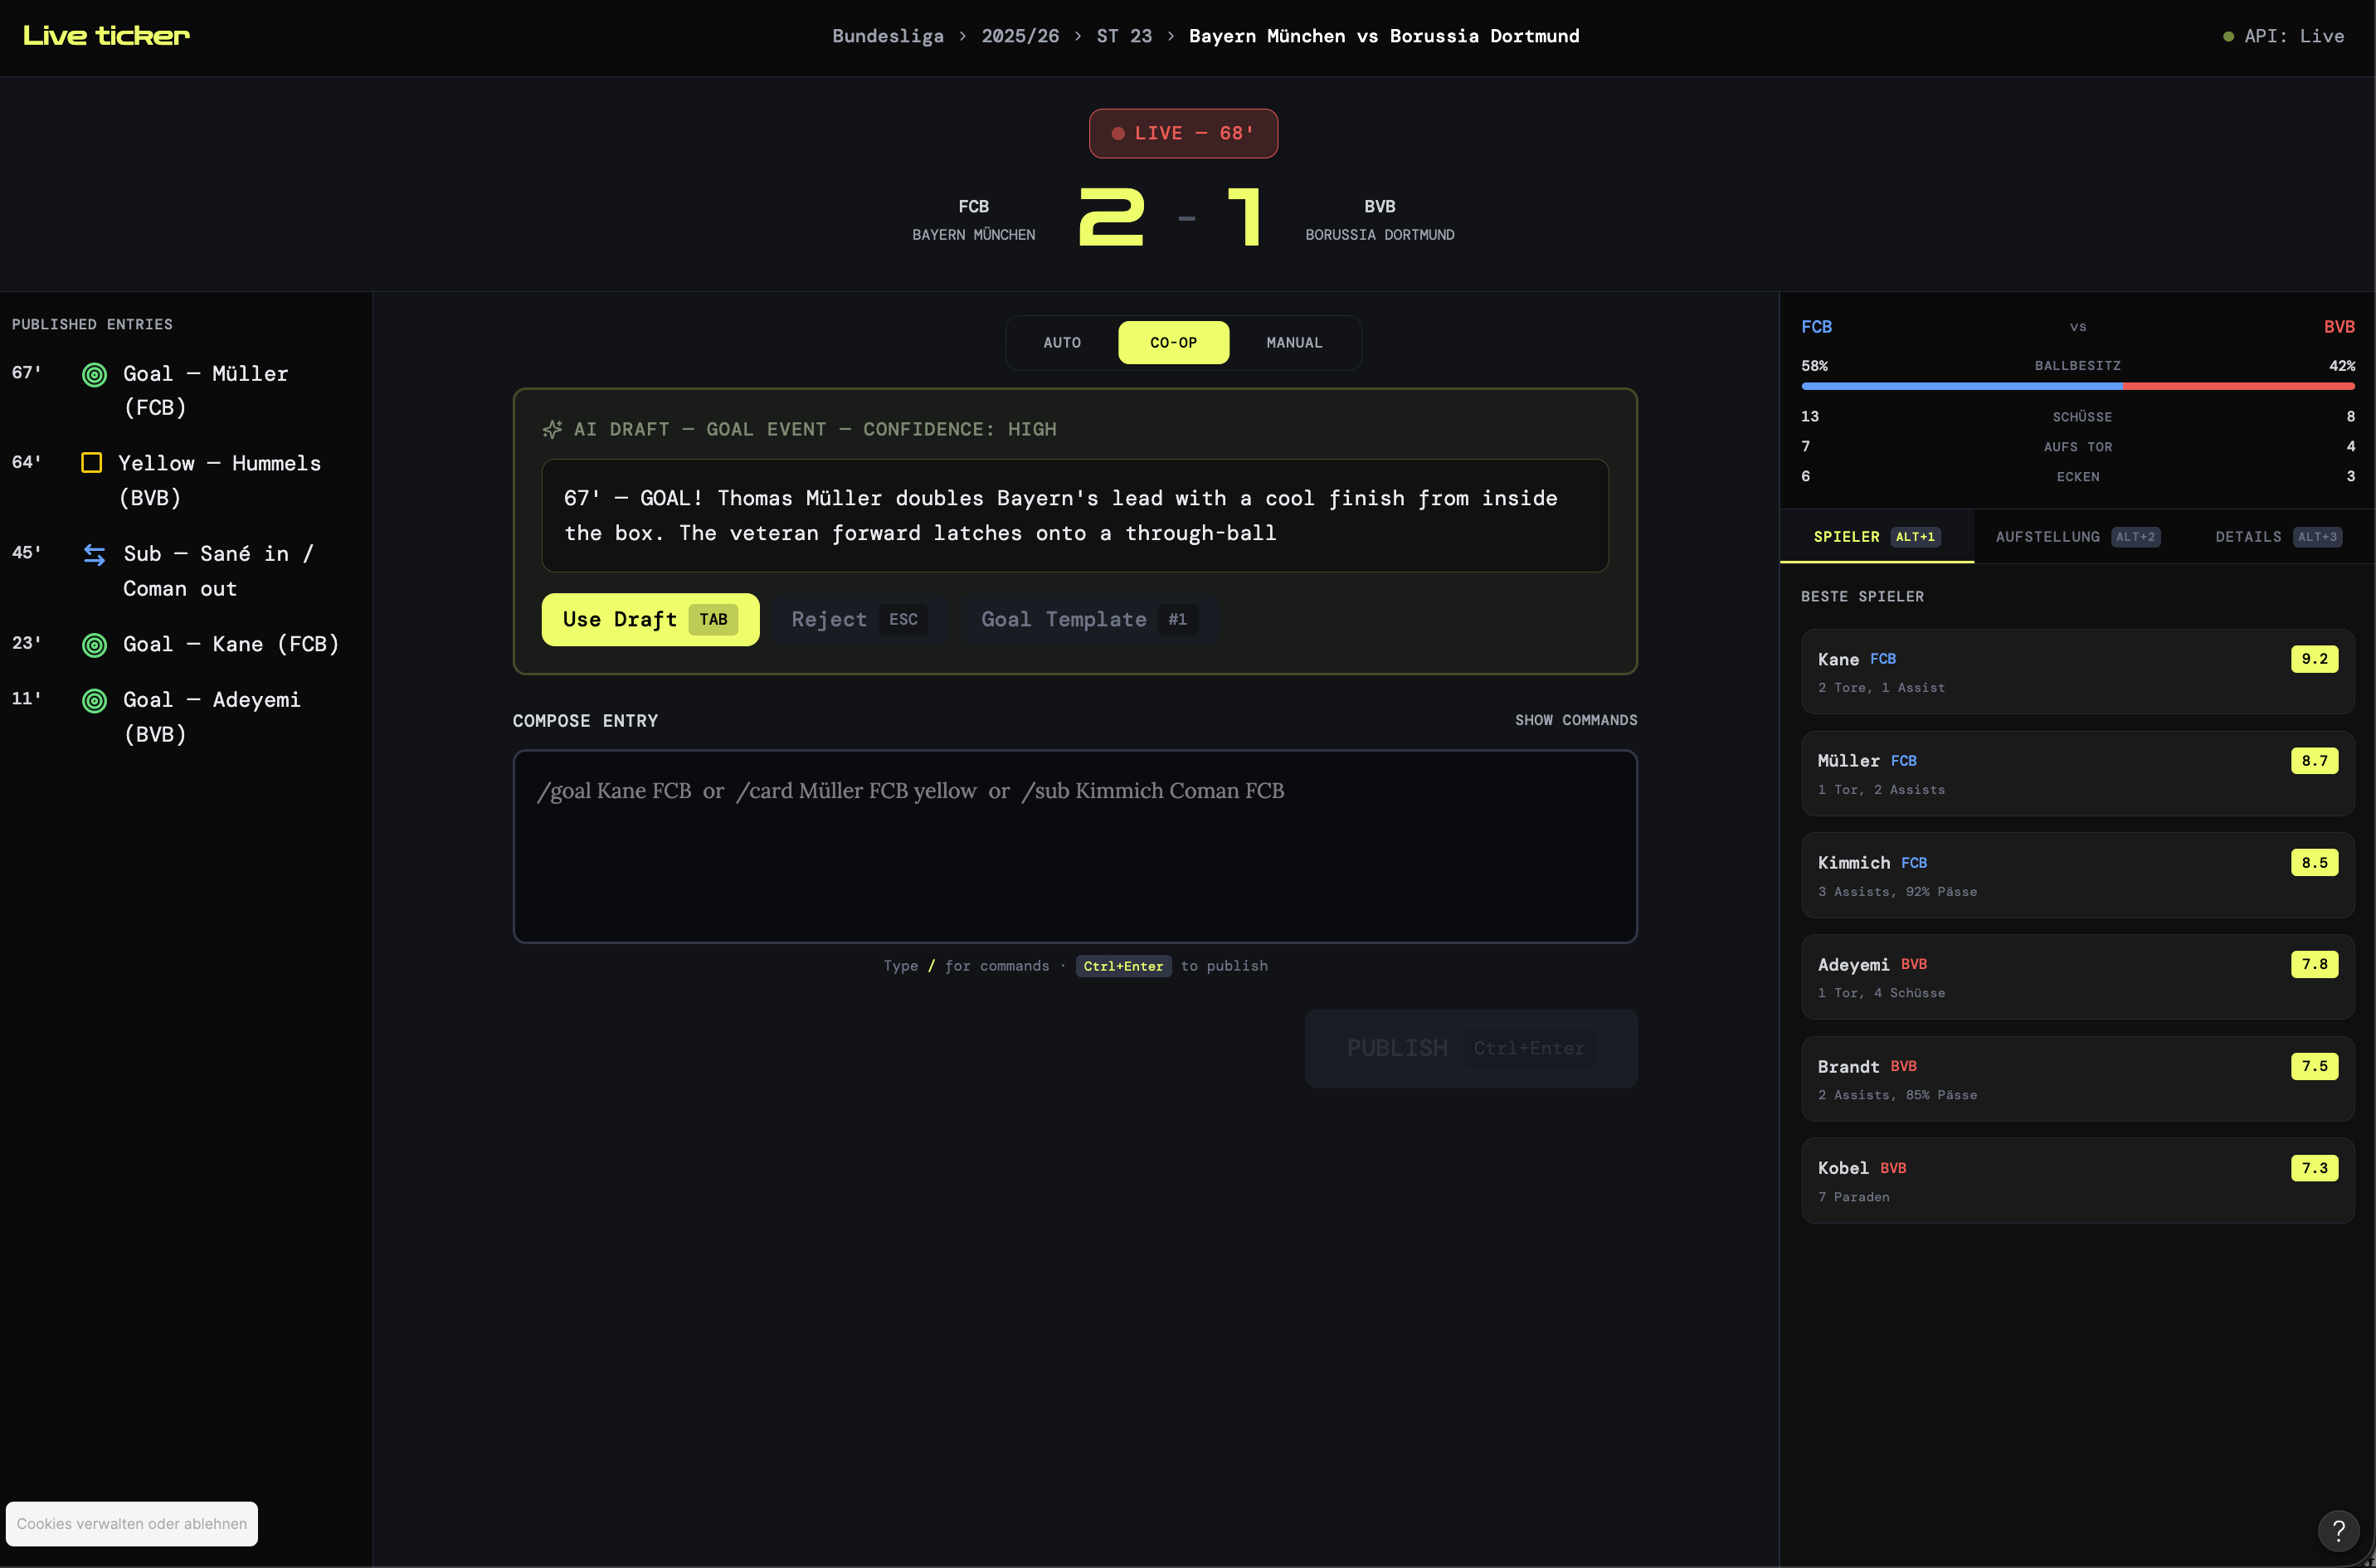
\includegraphics[width=\textwidth]{figma_wireframe.png}
\caption{Figma-Prototyp der Redaktionsoberfläche (Dreispalten-Layout)}
\label{fig:figma-wireframe}
\end{figure}

Im Rahmen des White-Label-Konzepts wurde darüber hinaus ein eigenes Applikationslogo entworfen und in beide Instanzen (\texttt{ef\_whitelabel} und \texttt{generic}) integriert.

\subsection{Teststrategie}\label{frontend-teststrategie}

Das Frontend wird auf drei Ebenen getestet: Utility-Funktionen (reine Transformations- und Berechnungslogik), Custom Hooks (Zustand und Seiteneffekte isoliert von der UI) und Komponenten (Rendering und Interaktionsverhalten). TypeScript-Typsicherheit ergänzt die Laufzeittests als statische Analyseschicht. Der \texttt{parseCommand}-Slash-Command-Parser erhält dabei besonders umfangreiche Testabdeckung, da er als einzige Schicht manuelle Redakteurseingaben ohne Backend-Validierung verarbeitet: ein Parsing-Fehler würde sich direkt in falsch klassierten Ticker-Einträgen niederschlagen. \textbf{Jest} wurde für Frontend-Tests gegenüber Vitest bevorzugt, da Jest in der bestehenden Projektkonfiguration nativ integriert ist und kein zusätzlicher Build-Stack eingeführt werden muss. Vitests Laufzeitvorteil wird erst bei deutlich größeren Test-Suites relevant. \textbf{Playwright} wurde für E2E-Tests gegenüber Cypress bevorzugt, da es keine Electron-Laufzeitabhängigkeit benötigt, Cross-Browser-Tests ohne Lizenzschranken ermöglicht und für responsive Mobile-Tests auf verschiedenen Viewports die geeignetere Wahl ist.



\section{Deployment-Konzept}\label{deployment-konzept}

Das Deployment-Modell folgt dem Stateless-Design-Prinzip (vgl. Abschnitt~\ref{cloud-deployment}): Backend, Frontend und Datenbank werden als drei voneinander unabhängige Dienste betrieben, die keinen prozesslokalen Zustand teilen. Konfiguration und Zugangsdaten werden ausschließlich als Umgebungsvariablen injiziert, sodass keine Secrets im Repository verbleiben.

Als PaaS-Anbieter wurde Render gegenüber Heroku, Railway und Fly.io gewählt. Render bietet nativen Docker-Support, automatische Deployments aus einem Git-Branch und einen kostenlosen Tier, der für den Evaluationszeitraum ohne Infrastrukturaufwand ausreicht. Heroku hat seinen kostenlosen Tier eingestellt; Railway und Fly.io erfordern mehr manuelle Konfiguration für statische Frontend-Builds. Die PostgreSQL-Datenbank wird als Managed Service betrieben, sodass Backups, Patches und Verbindungspooling außerhalb der Anwendungsverantwortung liegen. Die konkreten Deployment-Konfigurationen sind in Abschnitt~\ref{deployment} dokumentiert.

Die n8n-Workflow-Instanz wird für den Evaluationszeitraum lokal betrieben und über einen Tunnel für eingehende Webhooks erreichbar gemacht. Diese Entscheidung eliminiert Hosting-Kosten und erlaubt schnelle Workflow-Iteration ohne Redeploy-Zyklen — auf Kosten der Produktionsreife. Die Limitationen gegenüber einem Produktivbetrieb sind in Abschnitt~\ref{technische-einordnung} diskutiert.




